%**************************************************************************
% WSC 2026 Poster Extended Abstract
% A Simulation Testbed for Multi-Sensor DAA Perception Before Flight Test
% Uses the official WSC 2026 author kit (wscposterproc).
%**************************************************************************
\documentclass{wscposterproc}

\usepackage{graphicx}
\usepackage{booktabs}
\usepackage{caption}
\captionsetup{font=scriptsize,skip=2pt,labelfont=bf}
\usepackage{mathptmx}
\usepackage[T1]{fontenc}
\usepackage[pdftex,colorlinks=true,urlcolor=blue,citecolor=black,anchorcolor=black,linkcolor=black]{hyperref}

\begin{document}

\WSCpagesetup{Machado and Kuroswiski}

\title{A SIMULATION TESTBED FOR EVALUATING MULTI-SENSOR DETECT-AND-AVOID PERCEPTION BEFORE FLIGHT TEST}

\author{
Pedro Henrique Blatt Machado\\[2pt]
Instituto Tecnol\'ogico de Aeron\'autica (ITA), S\~ao Jos\'e dos Campos, SP, BRAZIL\\
\email{pedro.blatt@ita.br}
\and
Andr\'e Kuroswiski\\[2pt]
Instituto de Controle do Espa\c{c}o A\'ereo (ICEA), S\~ao Jos\'e dos Campos, SP, BRAZIL\\
\email{andre.kuroswiski@icea.gov.br}
}

\maketitle

\section*{ABSTRACT}
Flight-testing non-cooperative encounters is costly and cannot repeat an identical geometry across competing sensor suites, so the sensing envelope that determines detect-and-avoid warning time is rarely measured directly.
We present a simulation testbed built on Cosys-AirSim that generates repeatable encounters and indexes every radar, LiDAR, and camera observation to the same frame-level ground-truth intruder range, with detector labels derived automatically from segmentation.
A thirty-run campaign spanning approach geometry, weather, and lighting demonstrates the design questions the testbed answers before any flight: modality complementarity by range band, with vision peaking between twenty-five and one hundred meters while radar presence cueing spans all bands, lighting invariance, and whether one vision model generalizes across four camera configurations.
Results are simulator-specific and false-alarm rates are not measured; we position the testbed as the first stage of a staged validation path whose next step is quantifying simulation-to-reality transfer in flight.

\section{INTRODUCTION}
\label{sec:intro}
Detect-and-avoid (DAA) alerting logic such as DAIDALUS is commonly evaluated assuming intruder state is already available~\shortcite{nasa_wellclear,rtca_do365b}, leaving untested the sensing envelope that sets warning time against non-cooperative traffic without Automatic Dependent Surveillance--Broadcast (ADS-B).
Sensor Uncertainty Mitigation expands Well Clear volumes under noisy measurements~\cite{abramson2020sum}, but still needs modality-specific detection envelopes that flight test cannot supply at acceptable cost: an identical encounter cannot be repeated across competing sensor suites, and frame-level ground-truth range is unavailable simultaneously for radar, LiDAR, and camera.
High-fidelity multi-modal simulation can hold the encounter fixed and vary only the sensor chain~\shortcite{shah2018airsim,jansen2023cosys}.
Contributions: (i)~a Cosys-AirSim testbed with a frame-level ground-truth indexing contract; (ii)~a factorial encounter design over geometry, weather, and lighting; (iii)~a thirty-run demonstration of the pre-flight design questions the testbed answers; and (iv)~a declared staged path from synthetic campaign to instrumented flight test.

\section{SIMULATION TESTBED AND EXPERIMENT DESIGN}
\label{sec:method}
The testbed builds on Cosys-AirSim~\shortcite{jansen2023cosys} and is reusable for two reasons: detector labels are derived automatically from segmentation at zero annotation cost, and detections align by $(\texttt{run},\texttt{frame})$ to telemetry \texttt{dist\_xy\_m}, which makes cross-modal comparison fair.
Thirty runs vary approach azimuth, vertical separation, weather (clear, fog, rain, dust, snow), and lighting (day, dawn, dusk, night).
Modalities: an FMCW radar return-presence gate (no clutter, no classification); high-density LiDAR (OS128) and sparse LiDAR (VLP-16) with geometric clustering~\shortcite{ester1996dbscan}; and four forward EO cameras---standard ($1280{\times}960$, $120^\circ$), medium ($1280{\times}960$, $90^\circ$), narrow HD ($1920{\times}1080$, $65^\circ$), and low-cost wide ($640{\times}480$, $78^\circ$)---processed by a unified YOLOv8s~\shortcite{jocher2023yolo} trained on pooled segmentation-derived labels.
EO rates use any-camera-detects over 976 frames (30 runs); LiDAR and radar use 640 synchronized frames (29 runs).

\section{DEMONSTRATION STUDY}
\label{sec:results}
The campaign answers three pre-flight design questions that flight test cannot isolate at this scale.
Table~\ref{tab:bands}: EO peaks mid-range (91.1\% at 25--50\,m; 100\% at 50--100\,m), matching or exceeding dense LiDAR there; the drop below 25\,m is geometric and beyond 100\,m angular size collapses.
Radar stays at 100\% in every band as an upper-bound presence signal under a no-clutter gate.
Overall rates: radar 100\% (640/640), dense LiDAR 63.1\% (404/640), EO 49.7\% (485/976), sparse LiDAR 16.1\% (103/640).
Mean first-detection ranges are 116.9\,m (radar), 113.2\,m (dense LiDAR), and 79.3\,m (EO; not frame-aligned)---about 7.8\,s, 7.5\,s, and 5.3\,s of warning at 15\,m/s closure.
Radar and LiDAR are lighting-invariant; EO varies from 39.5\% (dawn) to 65.9\% (night).
Table~\ref{tab:cameras}: the unified model matches or slightly exceeds each per-lens specialist (mAP50 0.92--0.99); splits are small, so the low-cost score is not evidence that lower resolution is better.

\vspace{-4mm}
\noindent
\begin{minipage}[t]{0.48\textwidth}
\centering
\captionsetup{type=table,font=scriptsize,skip=1pt}
{\scriptsize
\begin{tabular}{@{}lcccc@{}}
\toprule
\textbf{Dist.\ (m)} & \textbf{EO} & \textbf{HD} & \textbf{Sp.} & \textbf{Rad.} \\
\midrule
0--10    & 55.6 & 77.6 & 29.9 & 100 \\
10--25   & 44.3 & 77.1 & 32.1 & 100 \\
25--50   & 91.1 & 67.7 & 16.5 & 100 \\
50--100  &100.0 & 55.4 & 11.2 & 100 \\
100--150 &  2.0 & 58.5 &  0.0 & 100 \\
150--250 &  0.0 &  6.7 &  0.0 & 100 \\
\bottomrule
\end{tabular}}
\caption{Detection rate (\%). EO: 976/30 runs. LiDAR/Radar: 640/29. Radar is return-presence only.}
\label{tab:bands}
\end{minipage}\hfill
\begin{minipage}[t]{0.50\textwidth}
\centering
\captionsetup{type=table,font=scriptsize,skip=1pt}
{\scriptsize
\begin{tabular}{@{}lcccc@{}}
\toprule
\textbf{Camera} & \textbf{FOV} & \textbf{$N$} & \textbf{Sp.} & \textbf{Un.} \\
\midrule
Narrow HD & $65^\circ$ & 41  & 0.91 & 0.92 \\
Medium    & $90^\circ$ & 54  & 0.96 & 0.97 \\
Low-cost  & $78^\circ$ & 37  & 0.99 & 0.99 \\
Pooled    & ---     & 170 & 0.96 & 0.97 \\
\bottomrule
\end{tabular}}
\caption{Per-camera mAP50 (Spec./Unif.). Standard forward is pooled only.}
\label{tab:cameras}
\end{minipage}

\vspace{-2mm}
Figure~\ref{fig:panels} stresses the same pipeline across environments inside simulation: camera optics in an unseen urban scene (left pair) and clear-day versus rain frames (right pair).
\vspace{-4mm}
\begin{figure}[htb]
\centering
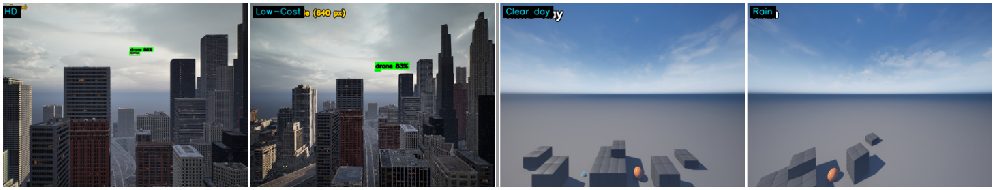
\includegraphics[width=0.98\textwidth]{../figures/wsc26_fig2.pdf}
\caption{Left pair: Narrow HD vs Low-Cost (urban). Right pair: Clear day vs rain. Within-sim stress tests.}
\label{fig:panels}
\end{figure}
\vspace{-5mm}

\section{CONCLUSIONS AND PATH TO FLIGHT TEST}
\label{sec:concl}
The testbed makes complementary, range-stratified sensing envelopes measurable before any aircraft leaves the ground: radar for early presence, dense LiDAR for geometry, and EO for mid-range classification with multi-lens generalization.
Validation stages: (i)~synthetic campaign, this work; (ii)~cross-environment stress inside simulation (Figure~\ref{fig:panels}); (iii)~hardware-in-the-loop; and (iv)~instrumented flight test quantifying the simulation-to-reality gap on these same metrics~\shortcite{tobin2017domain}.
False-alarm baselines and lateral/overtaking geometries remain open on that roadmap; current scenarios are frontal-biased.

\enlargethispage{36mm}
\vspace{-3mm}
{\fontsize{9}{10.5}\selectfont
\bibliographystyle{wsc}
\bibliography{wsc26refs}
}

\end{document}
